% ============================================================
%  Presentación — ¿Cómo estimar el índice de Theil con la GEIH?
%  Las figuras las generan los scripts de R en esta misma carpeta.
%  Compilar: pdflatex -> biber -> pdflatex -> pdflatex
% ============================================================
\documentclass[aspectratio=169]{beamer}

\usepackage[T1]{fontenc}
\usepackage[utf8]{inputenc}
\usepackage[spanish,es-nodecimaldot,es-noshorthands]{babel}
\usepackage{lmodern}
\usepackage{csquotes}
\usepackage[backend=biber,style=apa]{biblatex}
\addbibresource{references.bib}

\setbeamertemplate{navigation symbols}{}
\setbeamertemplate{footline}[frame number]

\title{¿Cómo estimar el índice de Theil con la GEIH?}
\subtitle{Desigualdad del ingreso laboral en Colombia, 2018--2026}
\author{Gabriel Salcedo \and Jerónimo Marín \and Isaac Suarez \and Santiago Velandia}
\institute{Universidad del Rosario --- Estadística}
\date{2026}

\begin{document}

\begin{frame}
  \titlepage
\end{frame}

\begin{frame}{Pregunta}
  % TODO: la pregunta de investigación de la primera entrega
\end{frame}

\begin{frame}{Cuatro estimadores del índice de Theil}
  \begin{itemize}
    \item A: con factor de expansión
    \item B: sin factor de expansión
    \item C: lognormal por momentos
    \item D: lognormal por máxima verosimilitud
  \end{itemize}
\end{frame}

\begin{frame}{Hipótesis}
  % TODO: H1, H2 y H3 en una línea cada una
\end{frame}

\begin{frame}{Datos: GEIH 2018--2026, enero a junio}
  % TODO: población y depuración (Tabla 2 de la primera entrega)
\end{frame}

\begin{frame}{¿Quiénes son los ocupados?}
  \centering
  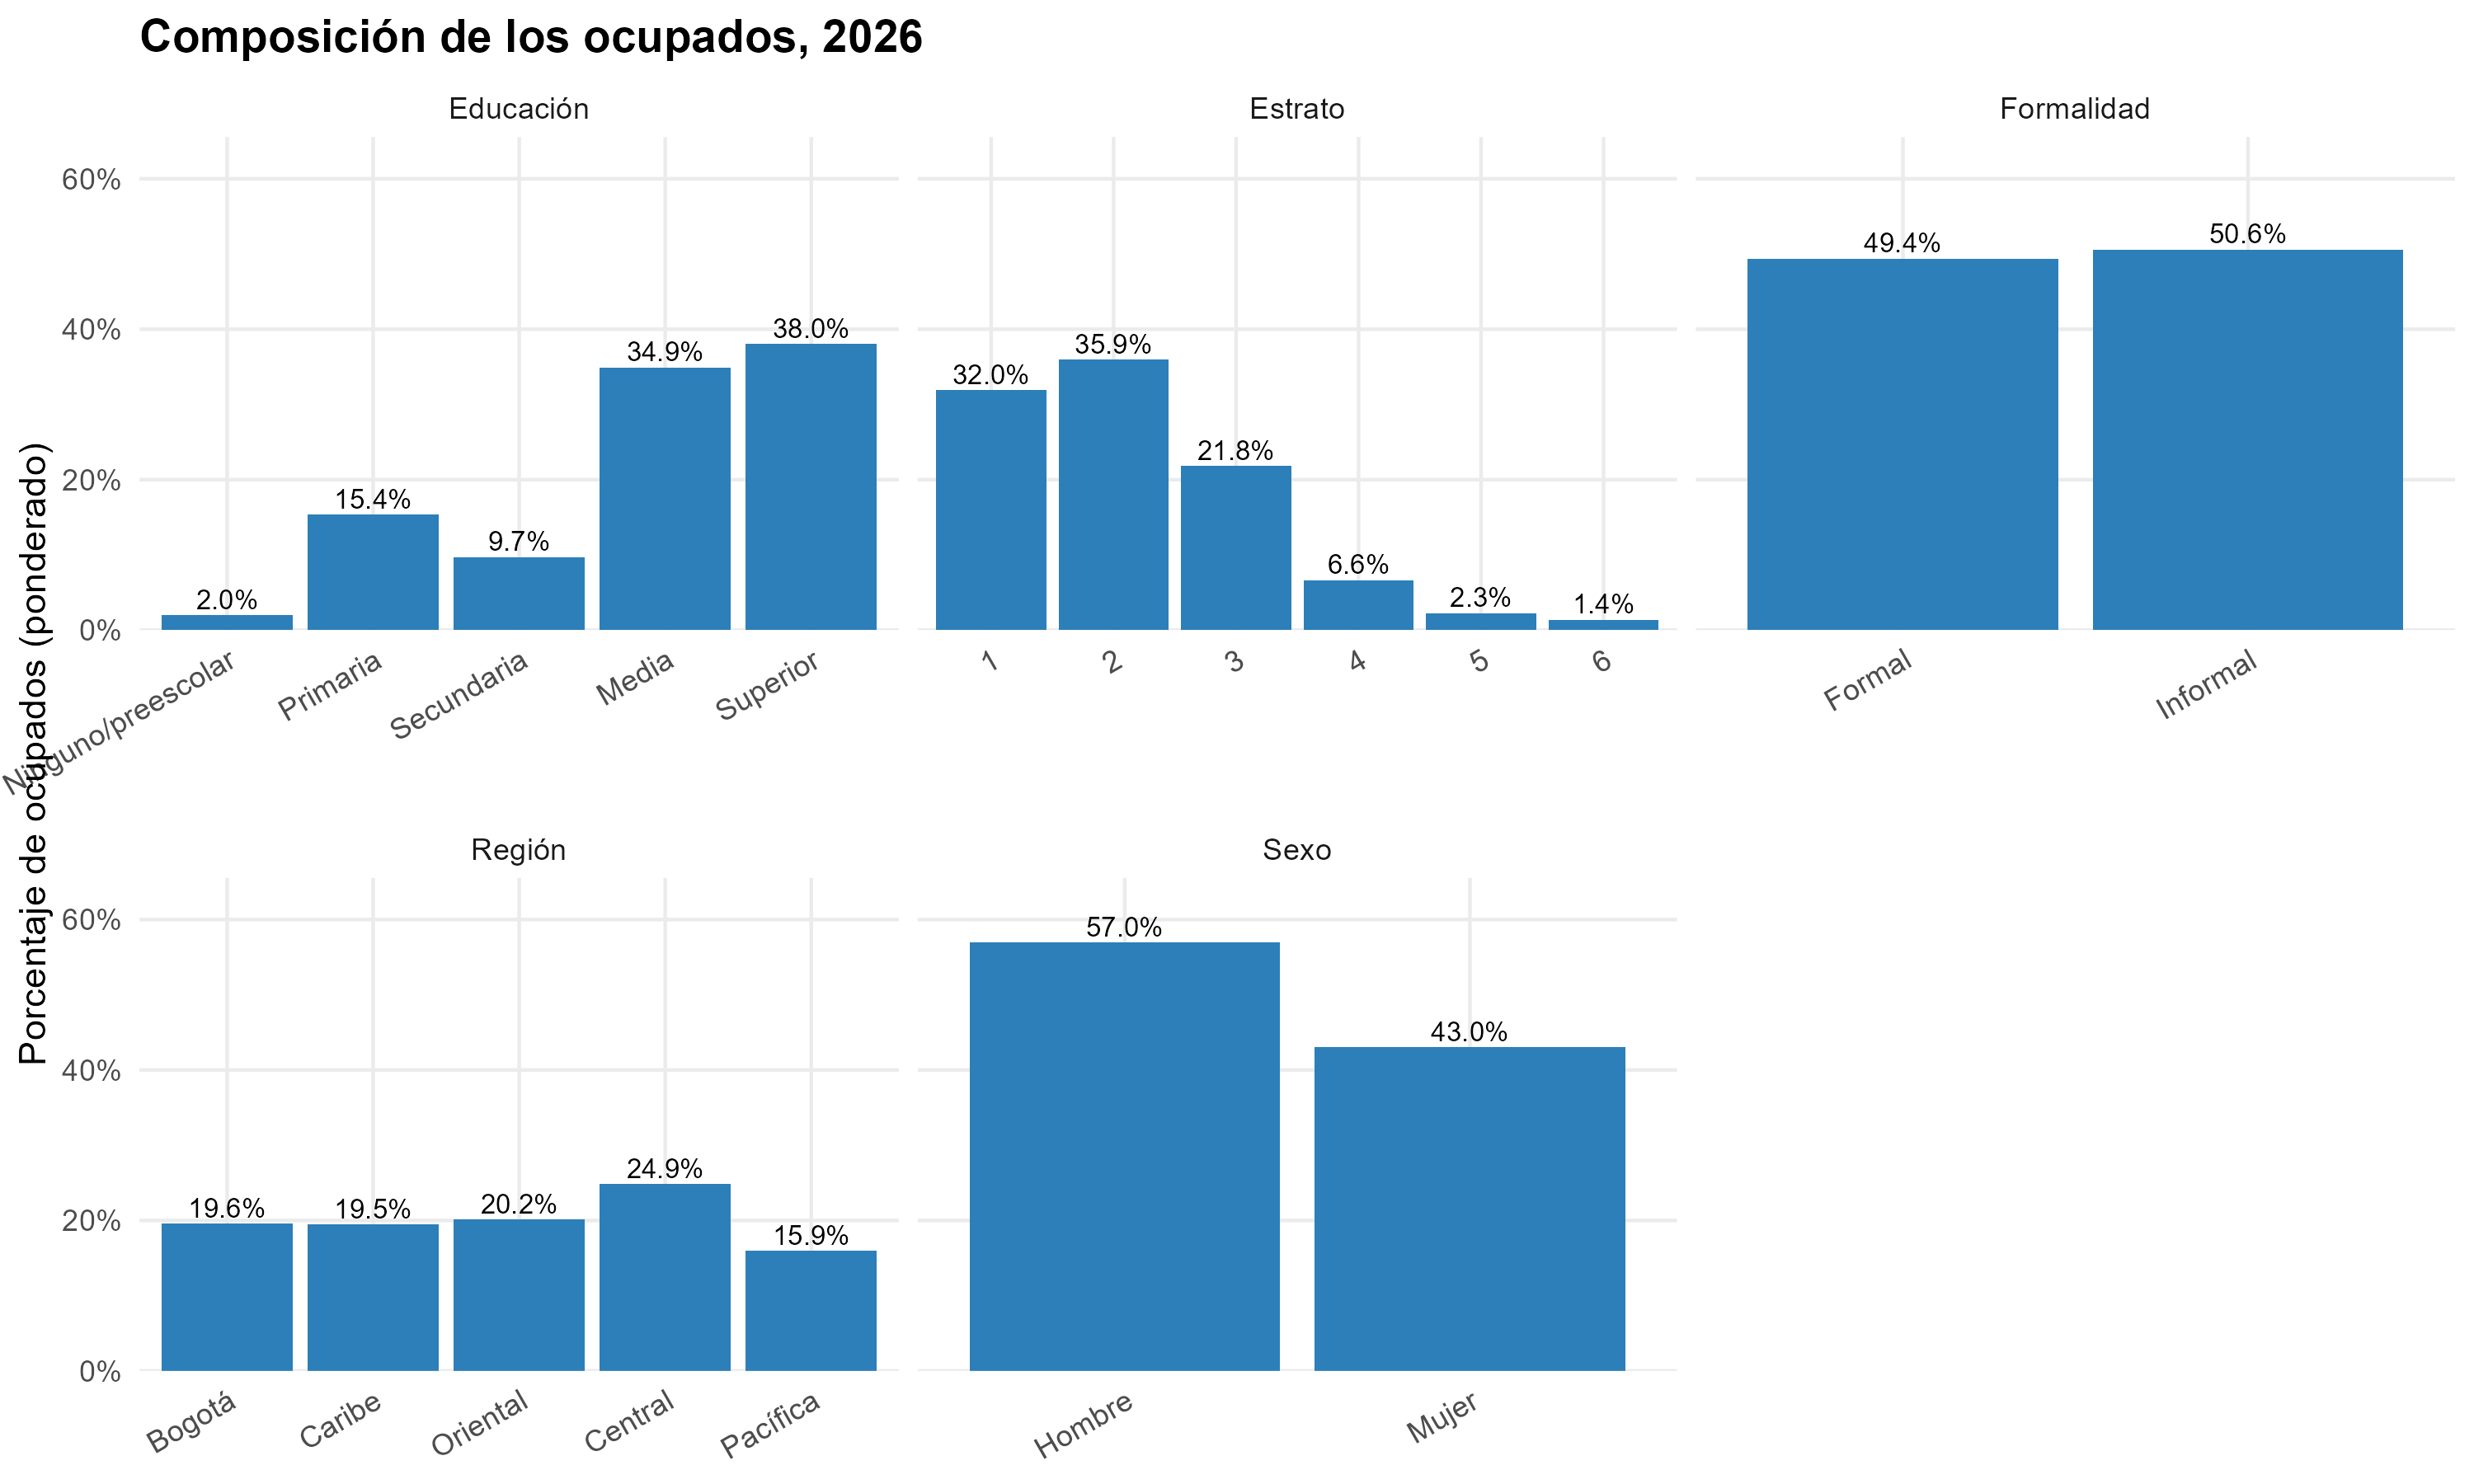
\includegraphics[height=0.8\textheight]{fig_barras_cualitativas.png}
\end{frame}

\begin{frame}{Distribución del ingreso}
  \centering
  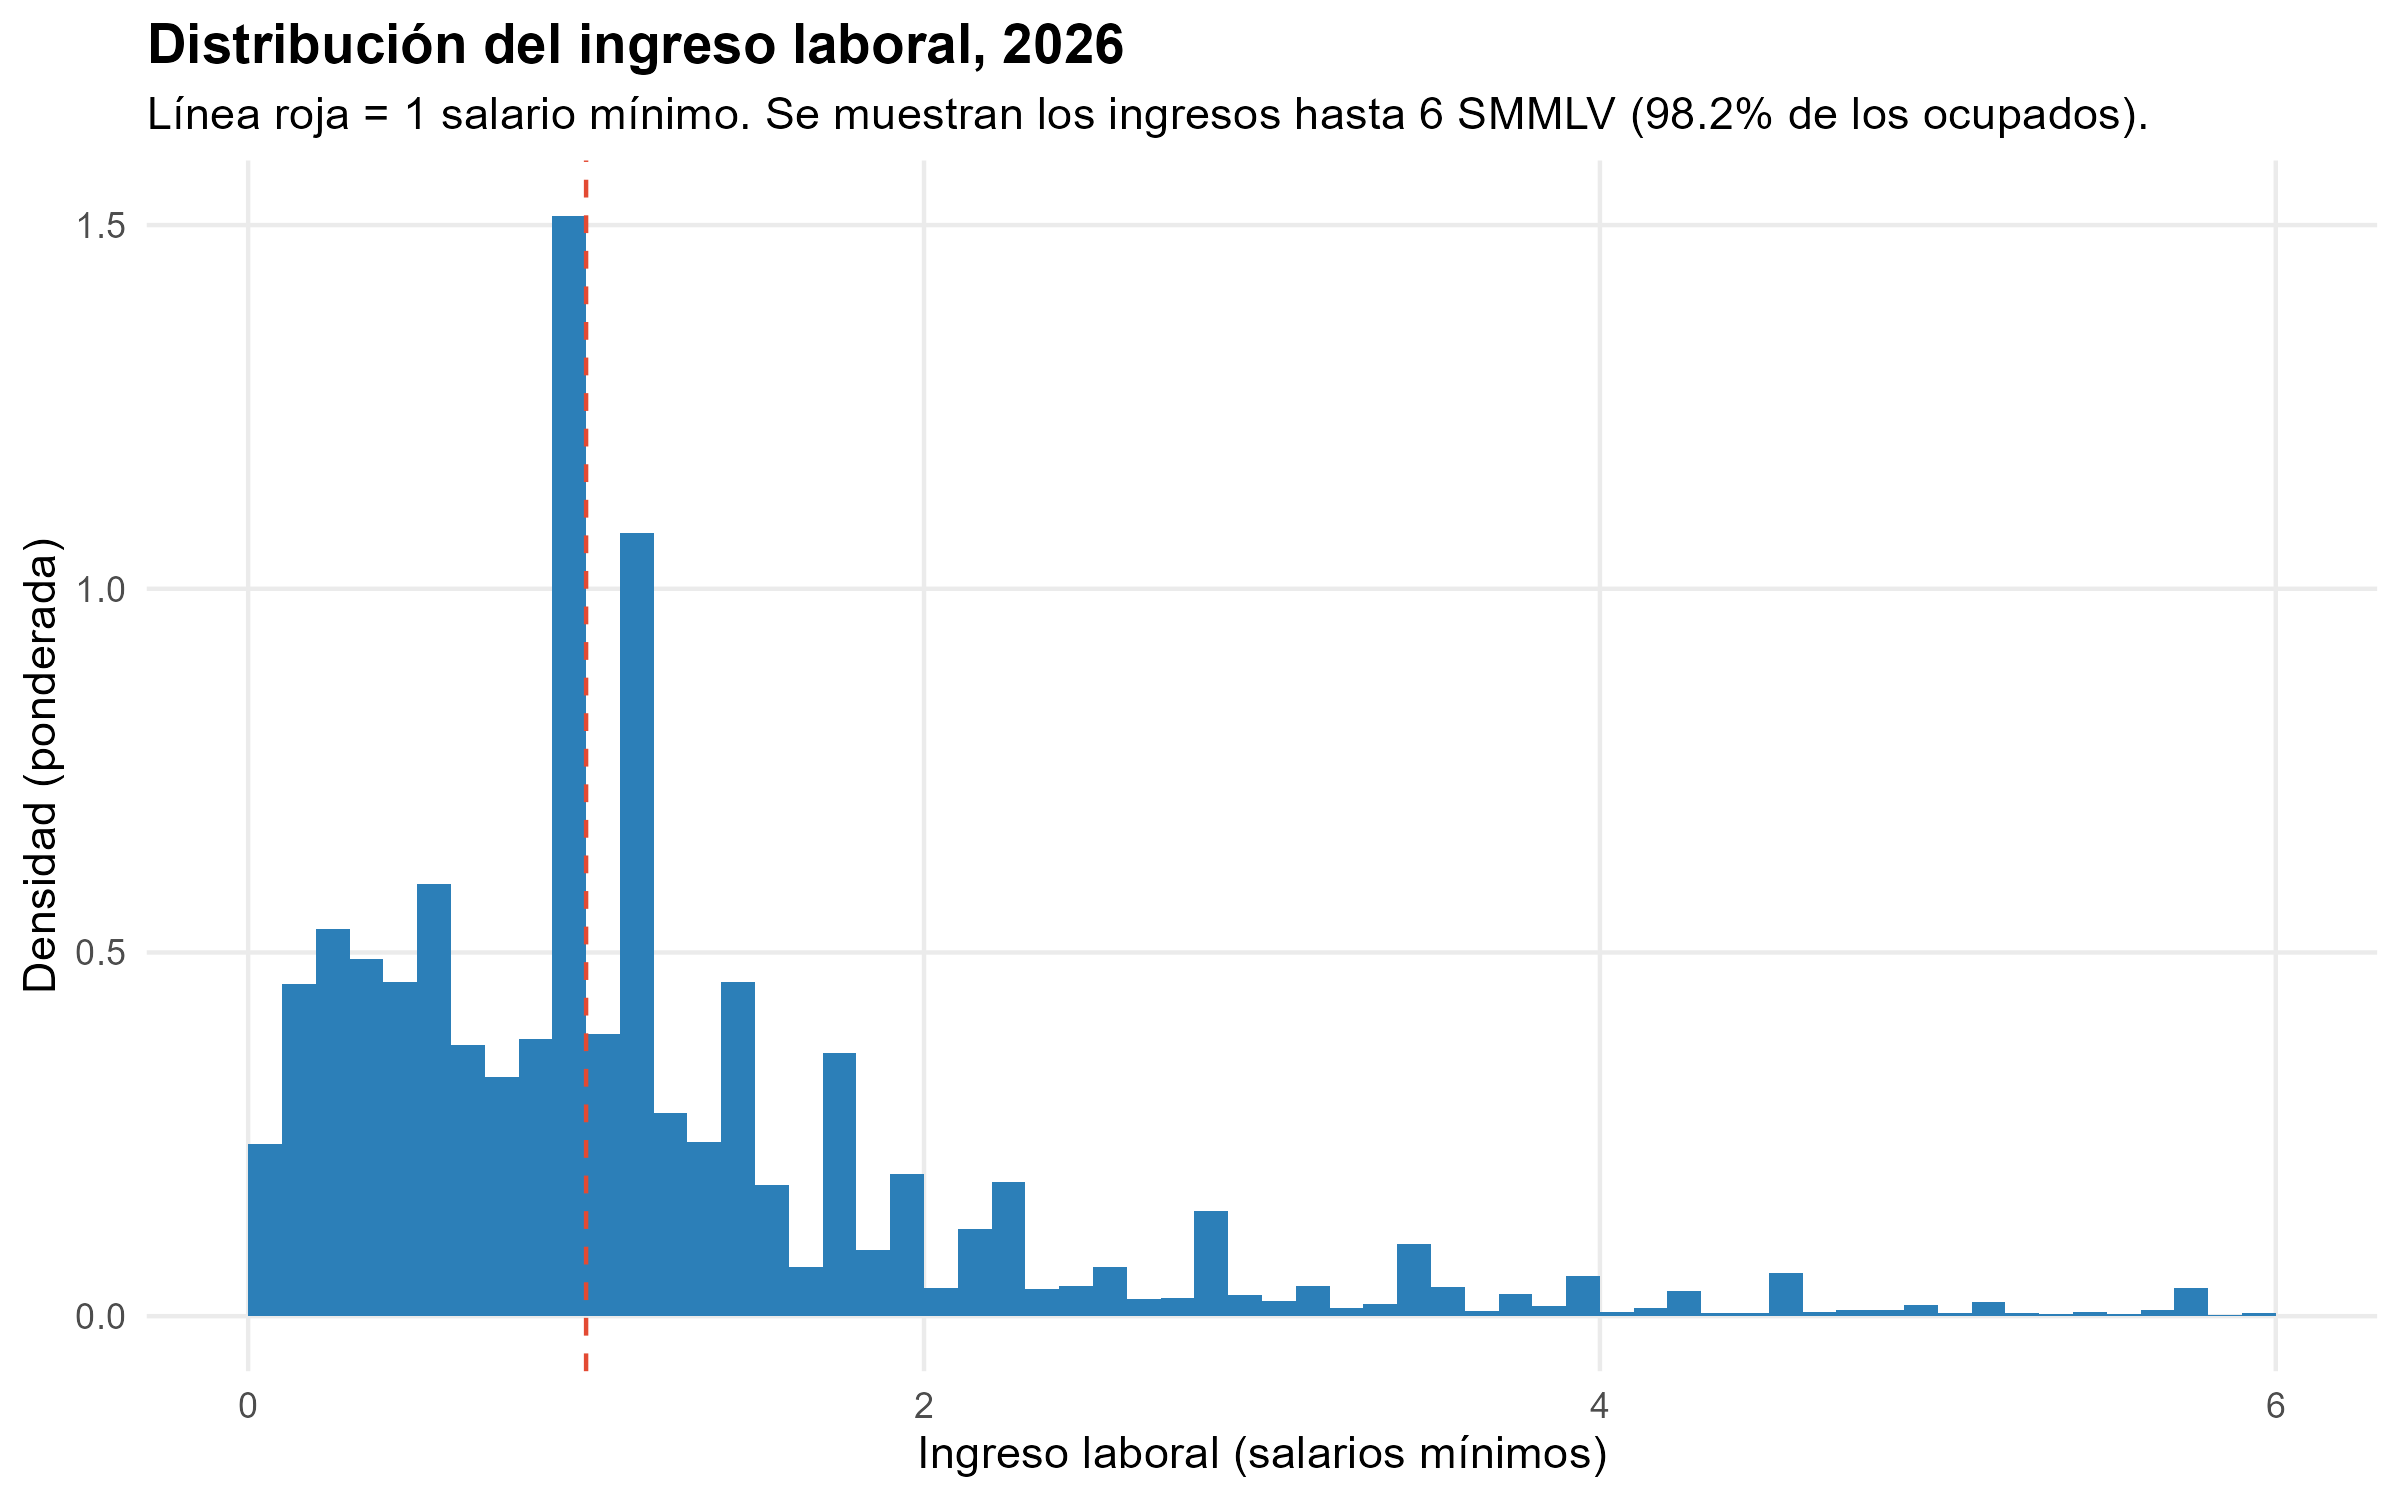
\includegraphics[height=0.8\textheight]{fig_histograma_ingreso.png}
\end{frame}

\begin{frame}{¿Es lognormal el ingreso?}
  \centering
  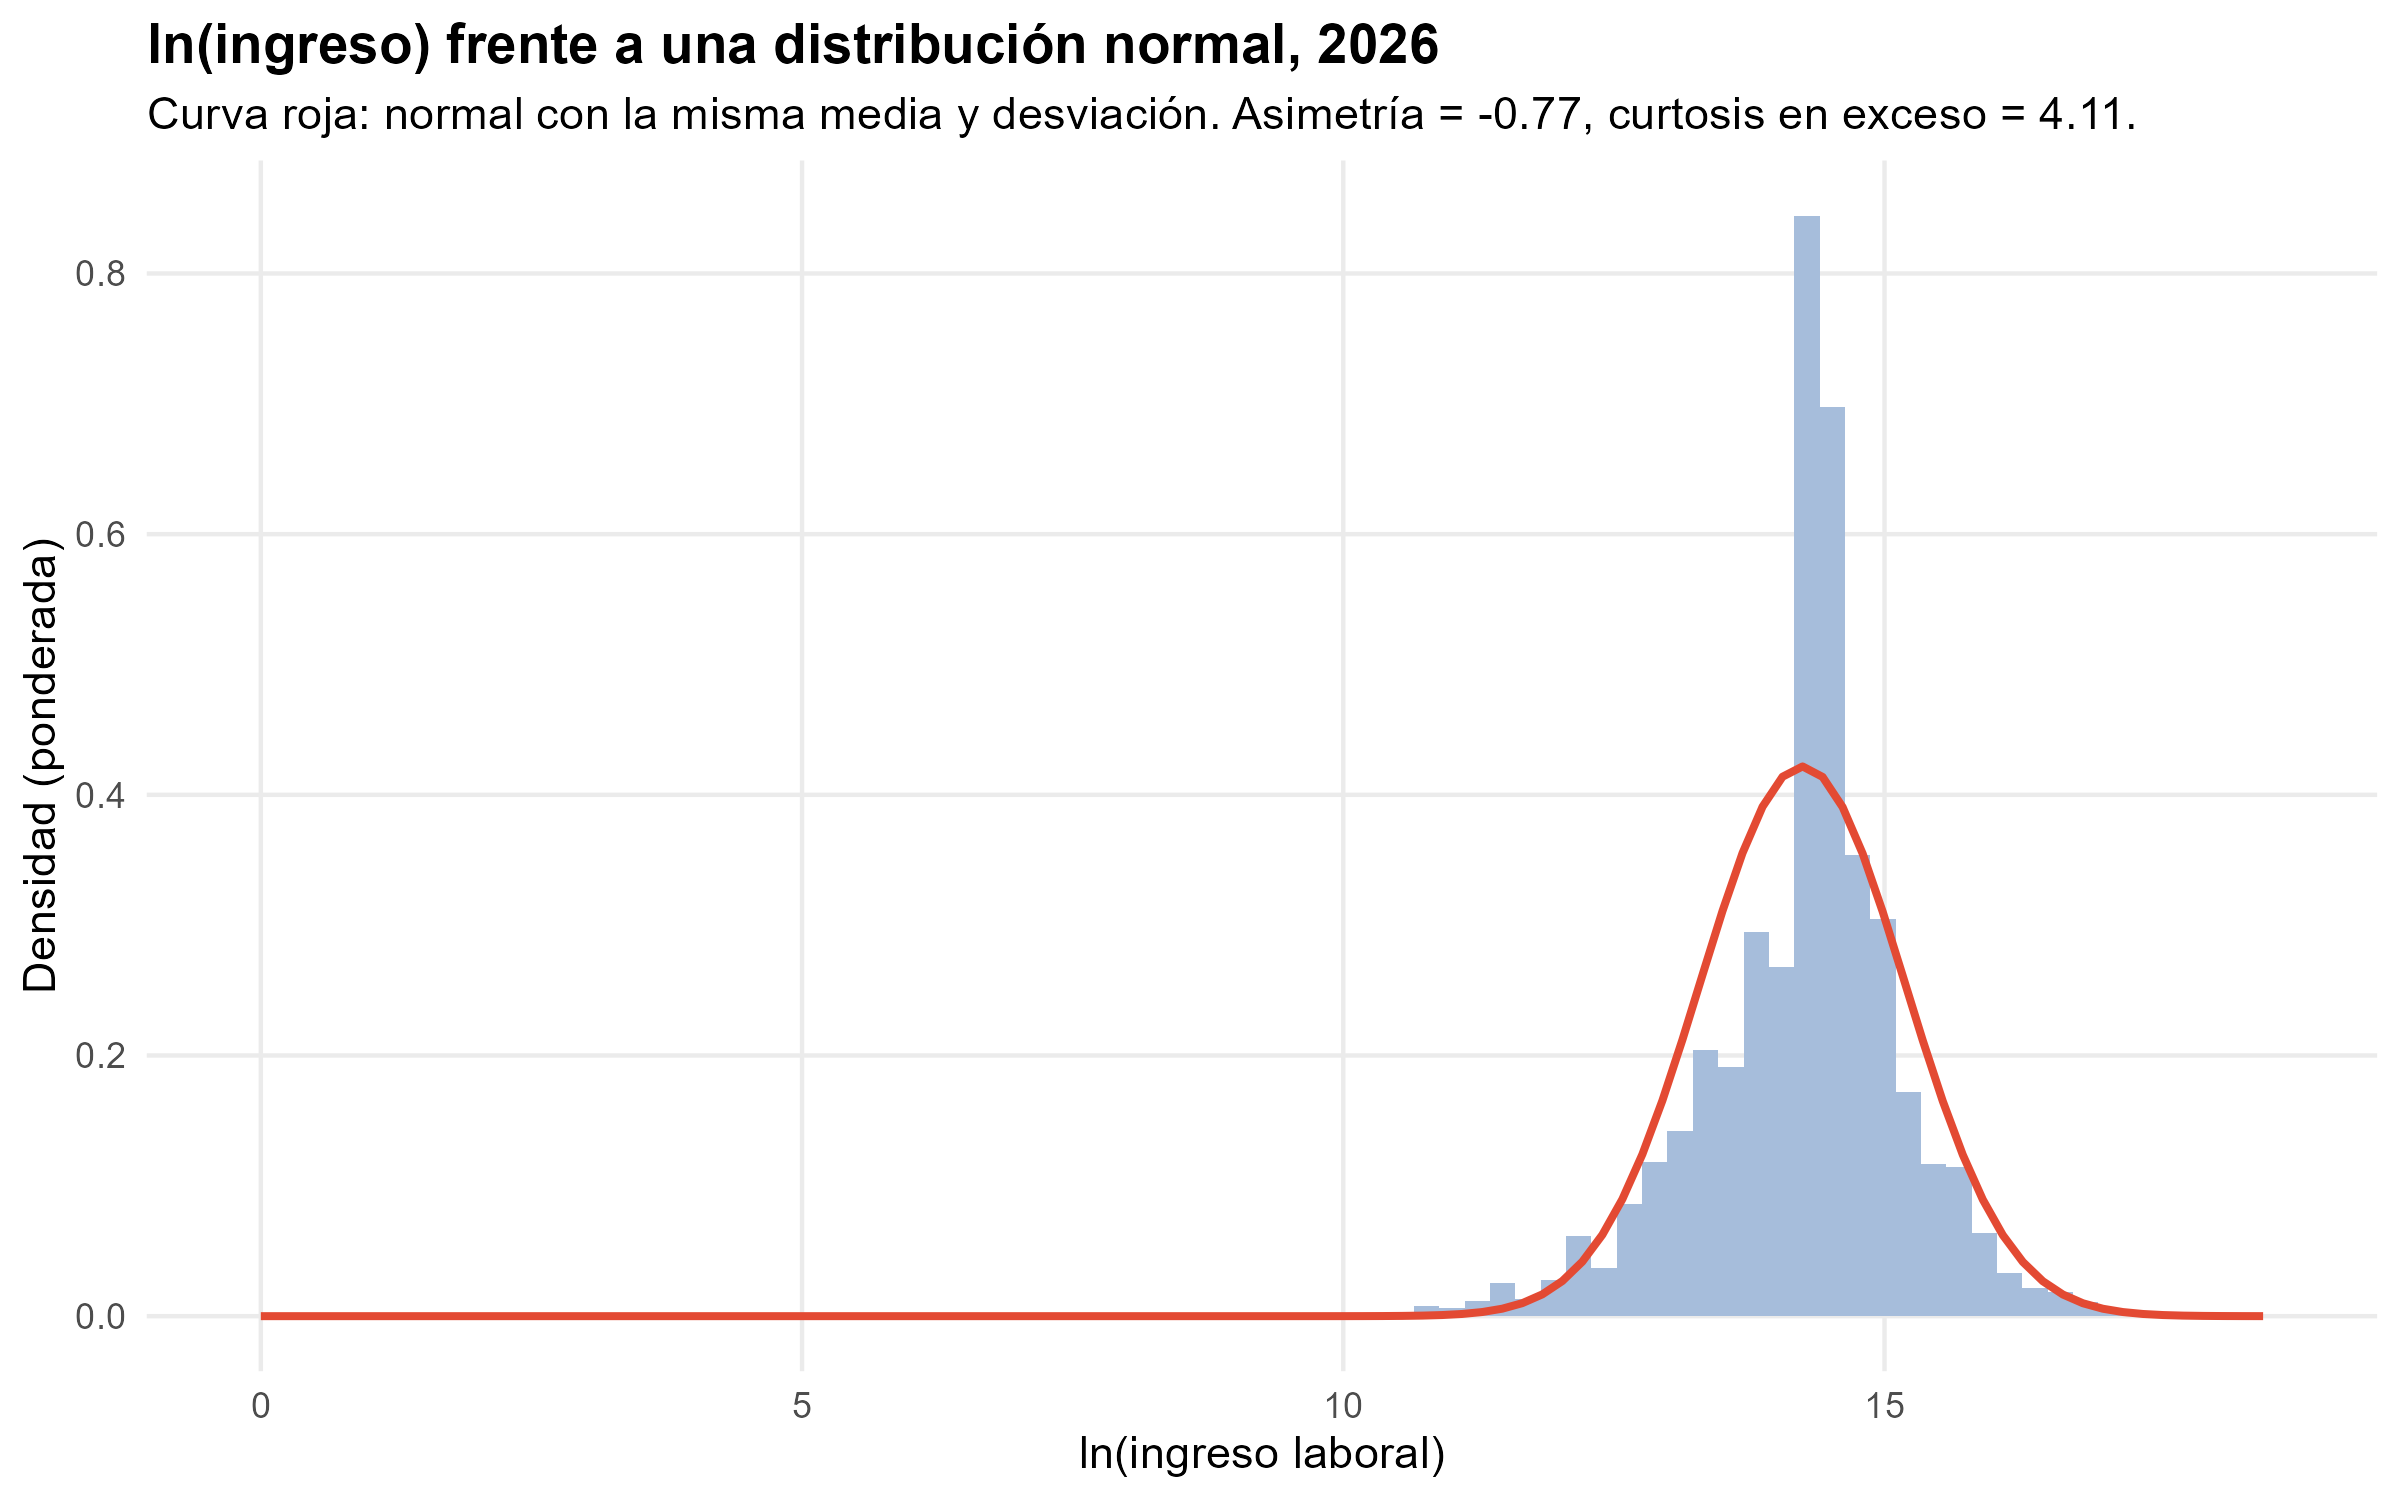
\includegraphics[height=0.8\textheight]{fig_ln_ingreso_normal.png}
\end{frame}

\begin{frame}{Ingreso por grupo}
  \centering
  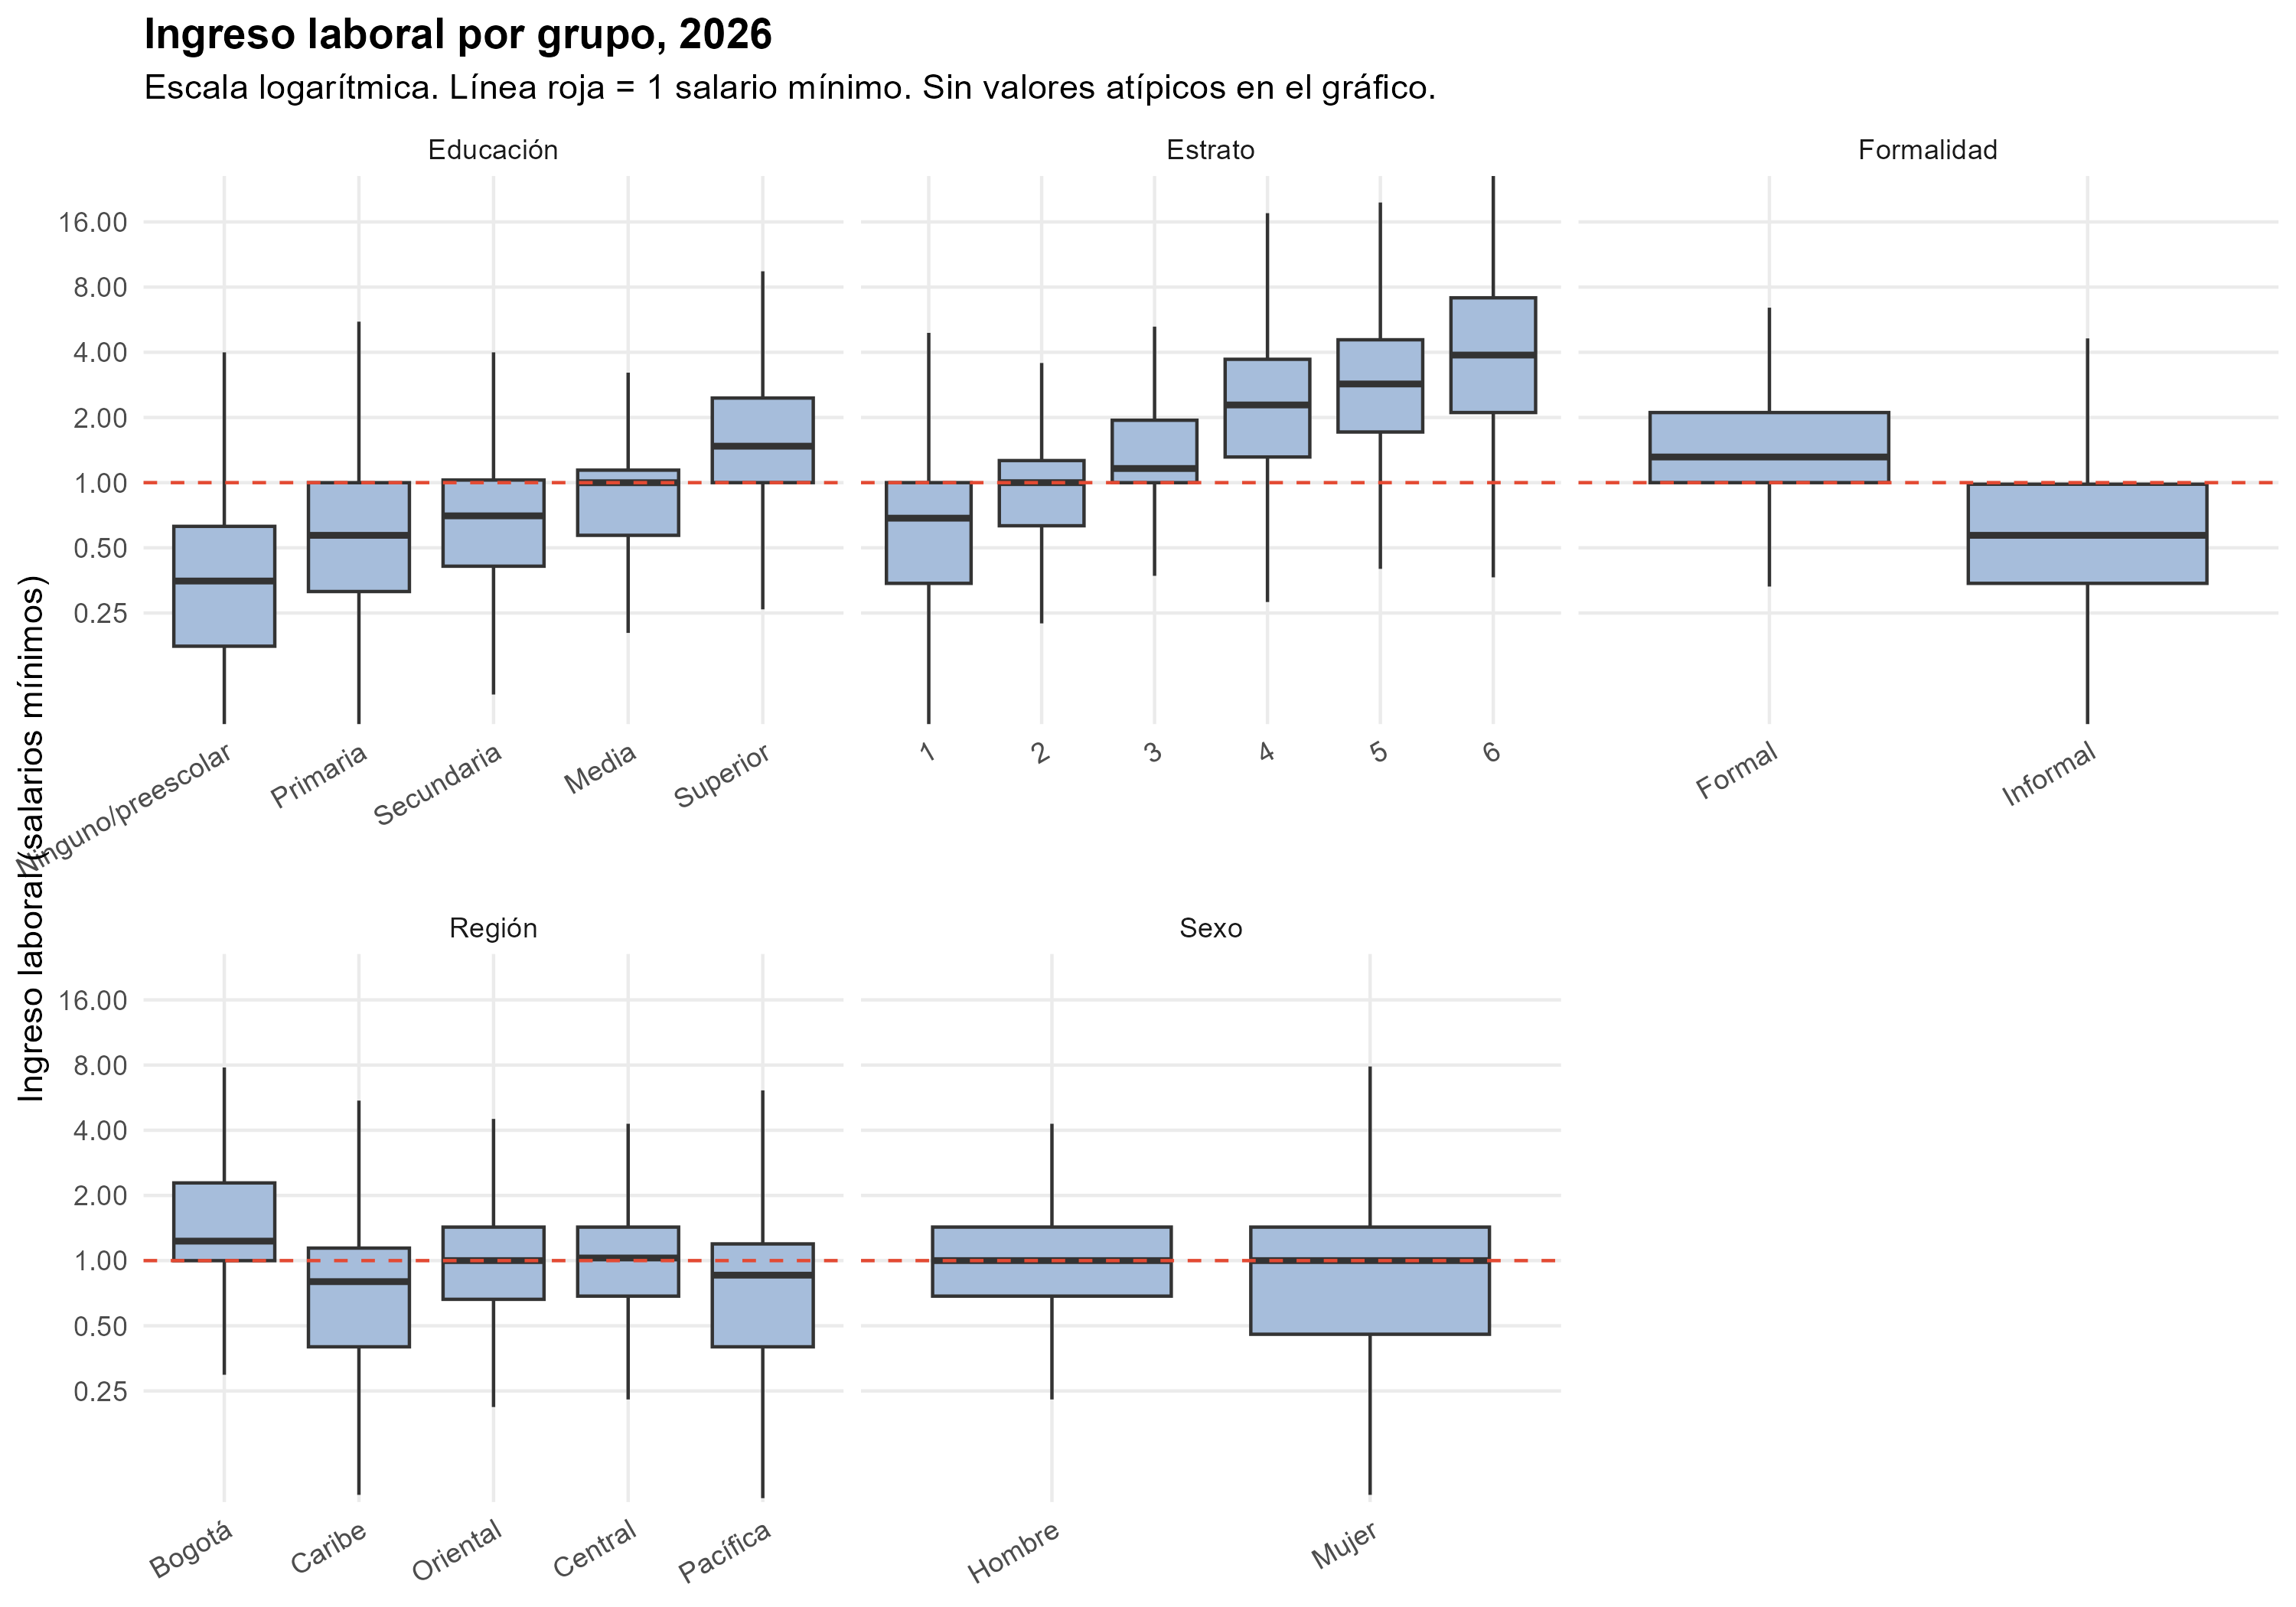
\includegraphics[height=0.8\textheight]{fig_boxplot_ingreso_grupo.png}
\end{frame}

\begin{frame}{Simulación: ECM según el tamaño de muestra (H1)}
  \centering
  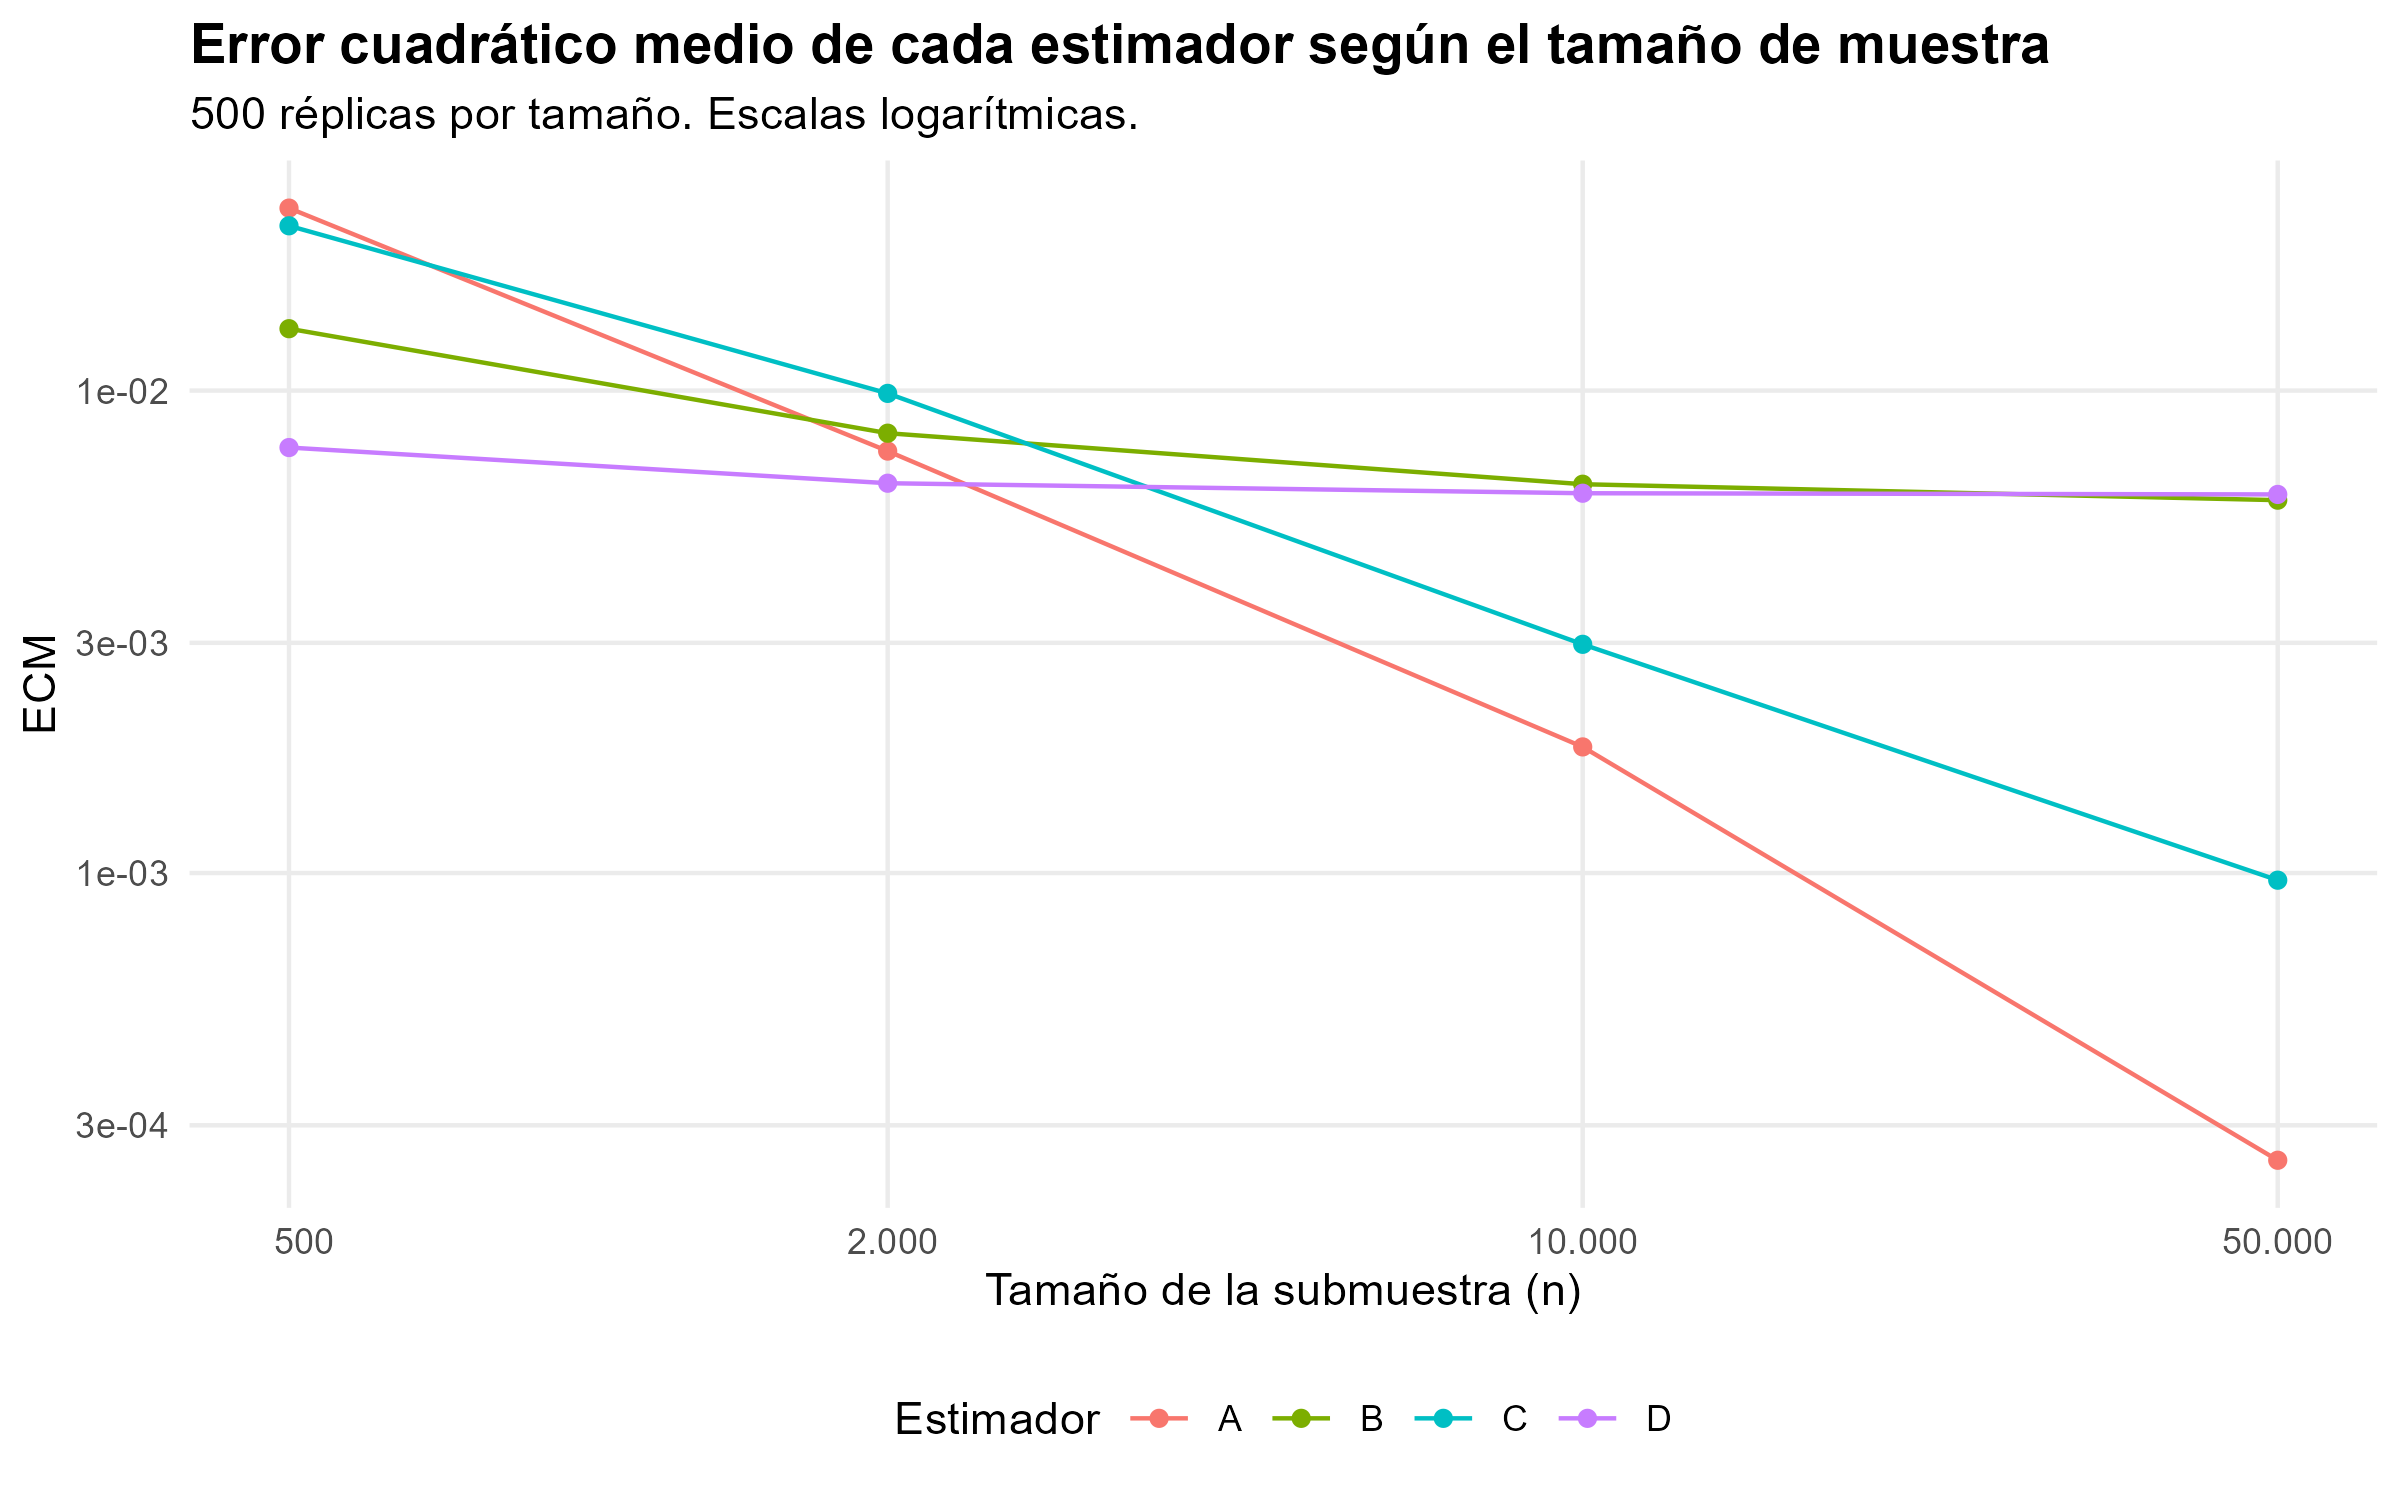
\includegraphics[height=0.8\textheight]{fig_simulacion_ecm.png}
\end{frame}

\begin{frame}{Simulación: 500 estimaciones con n = 50.000}
  \centering
  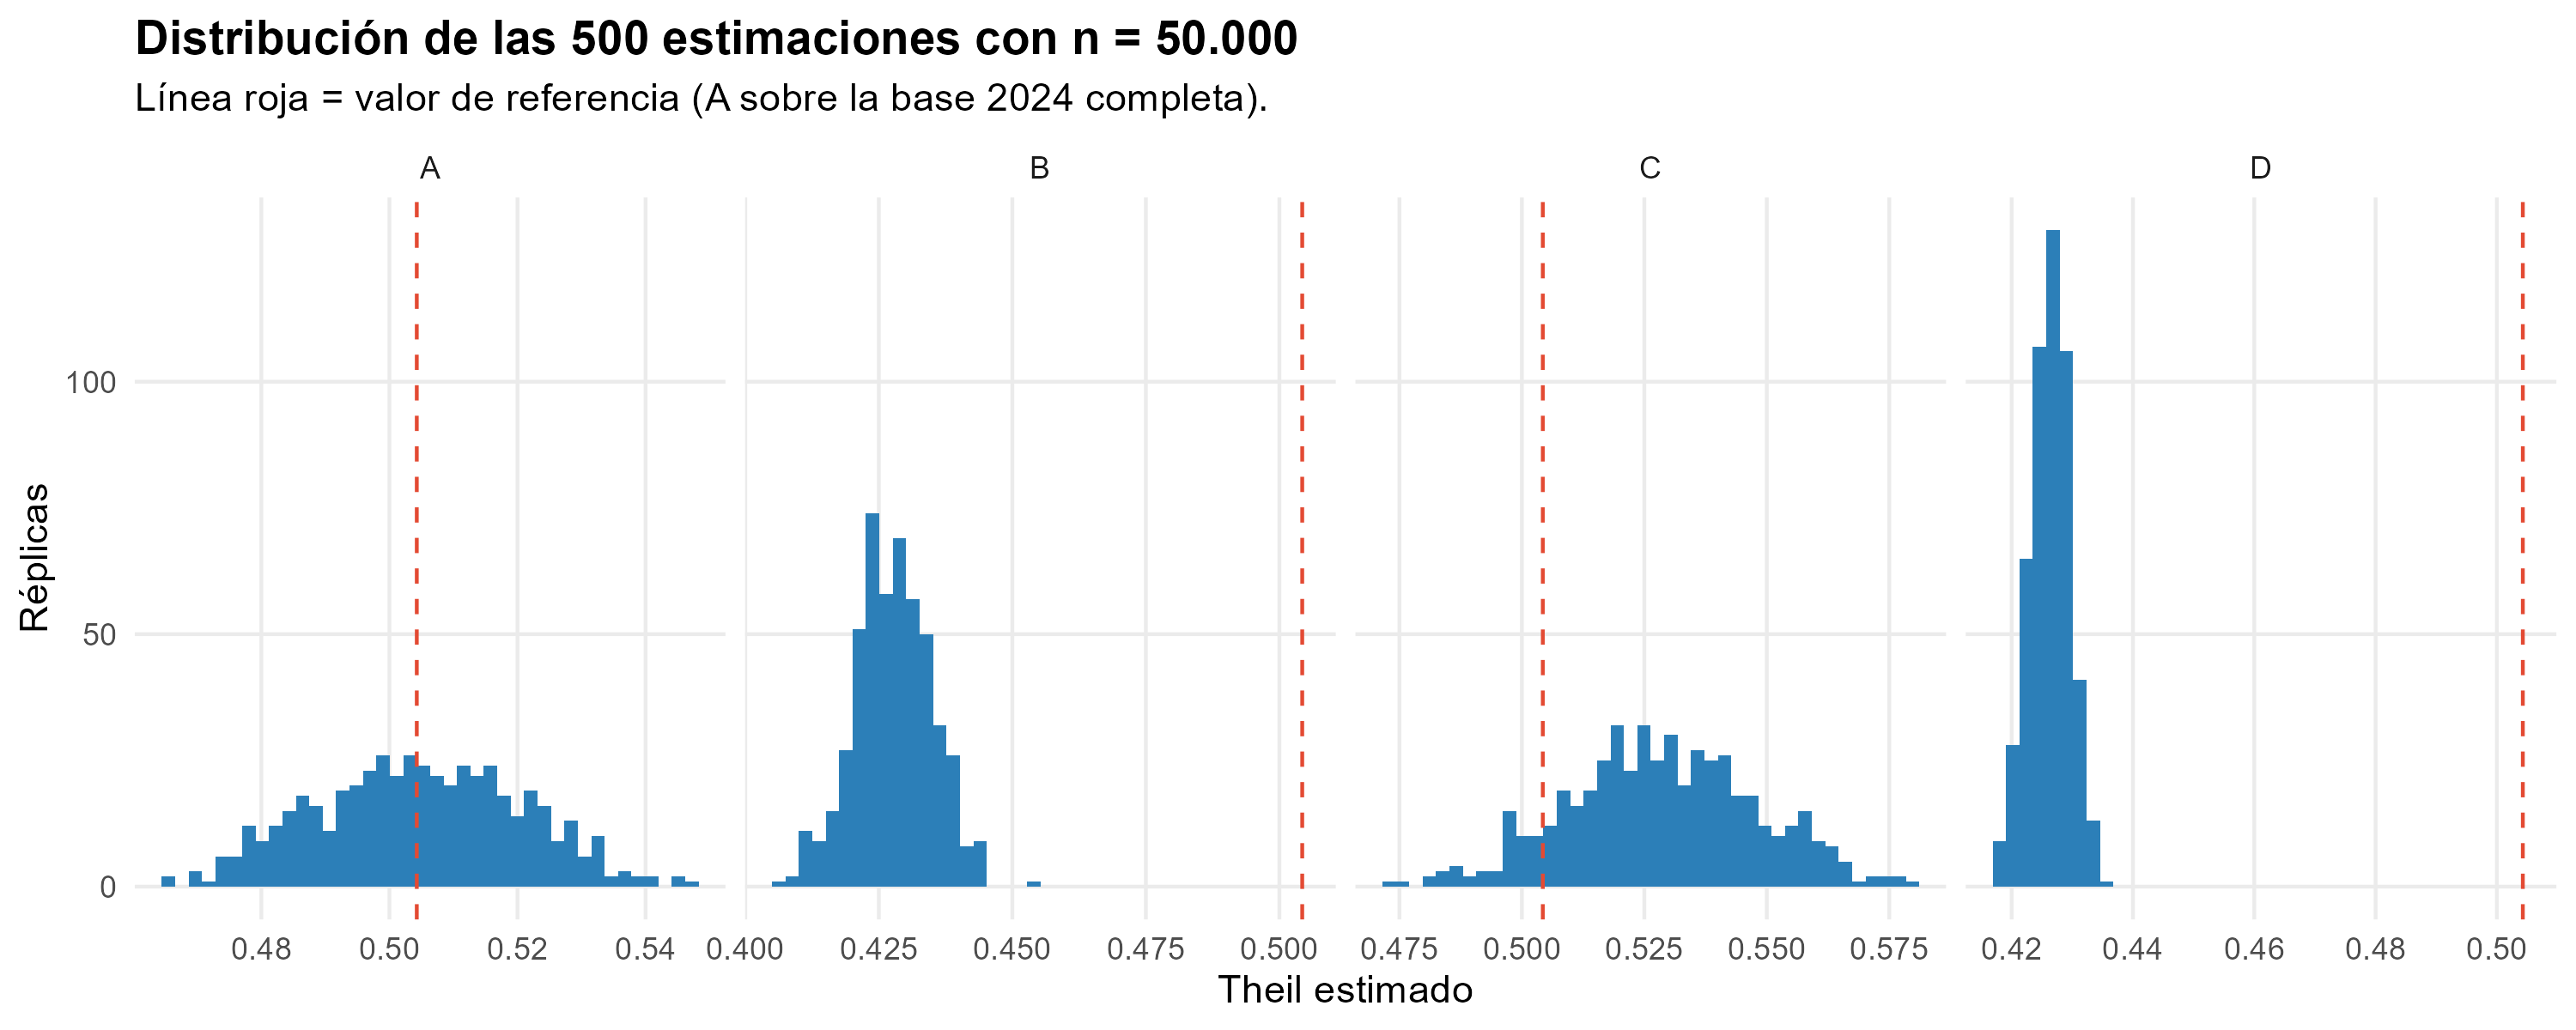
\includegraphics[width=\textwidth]{fig_simulacion_distribucion.png}
\end{frame}

\begin{frame}{Theil anual (H3)}
  \centering
  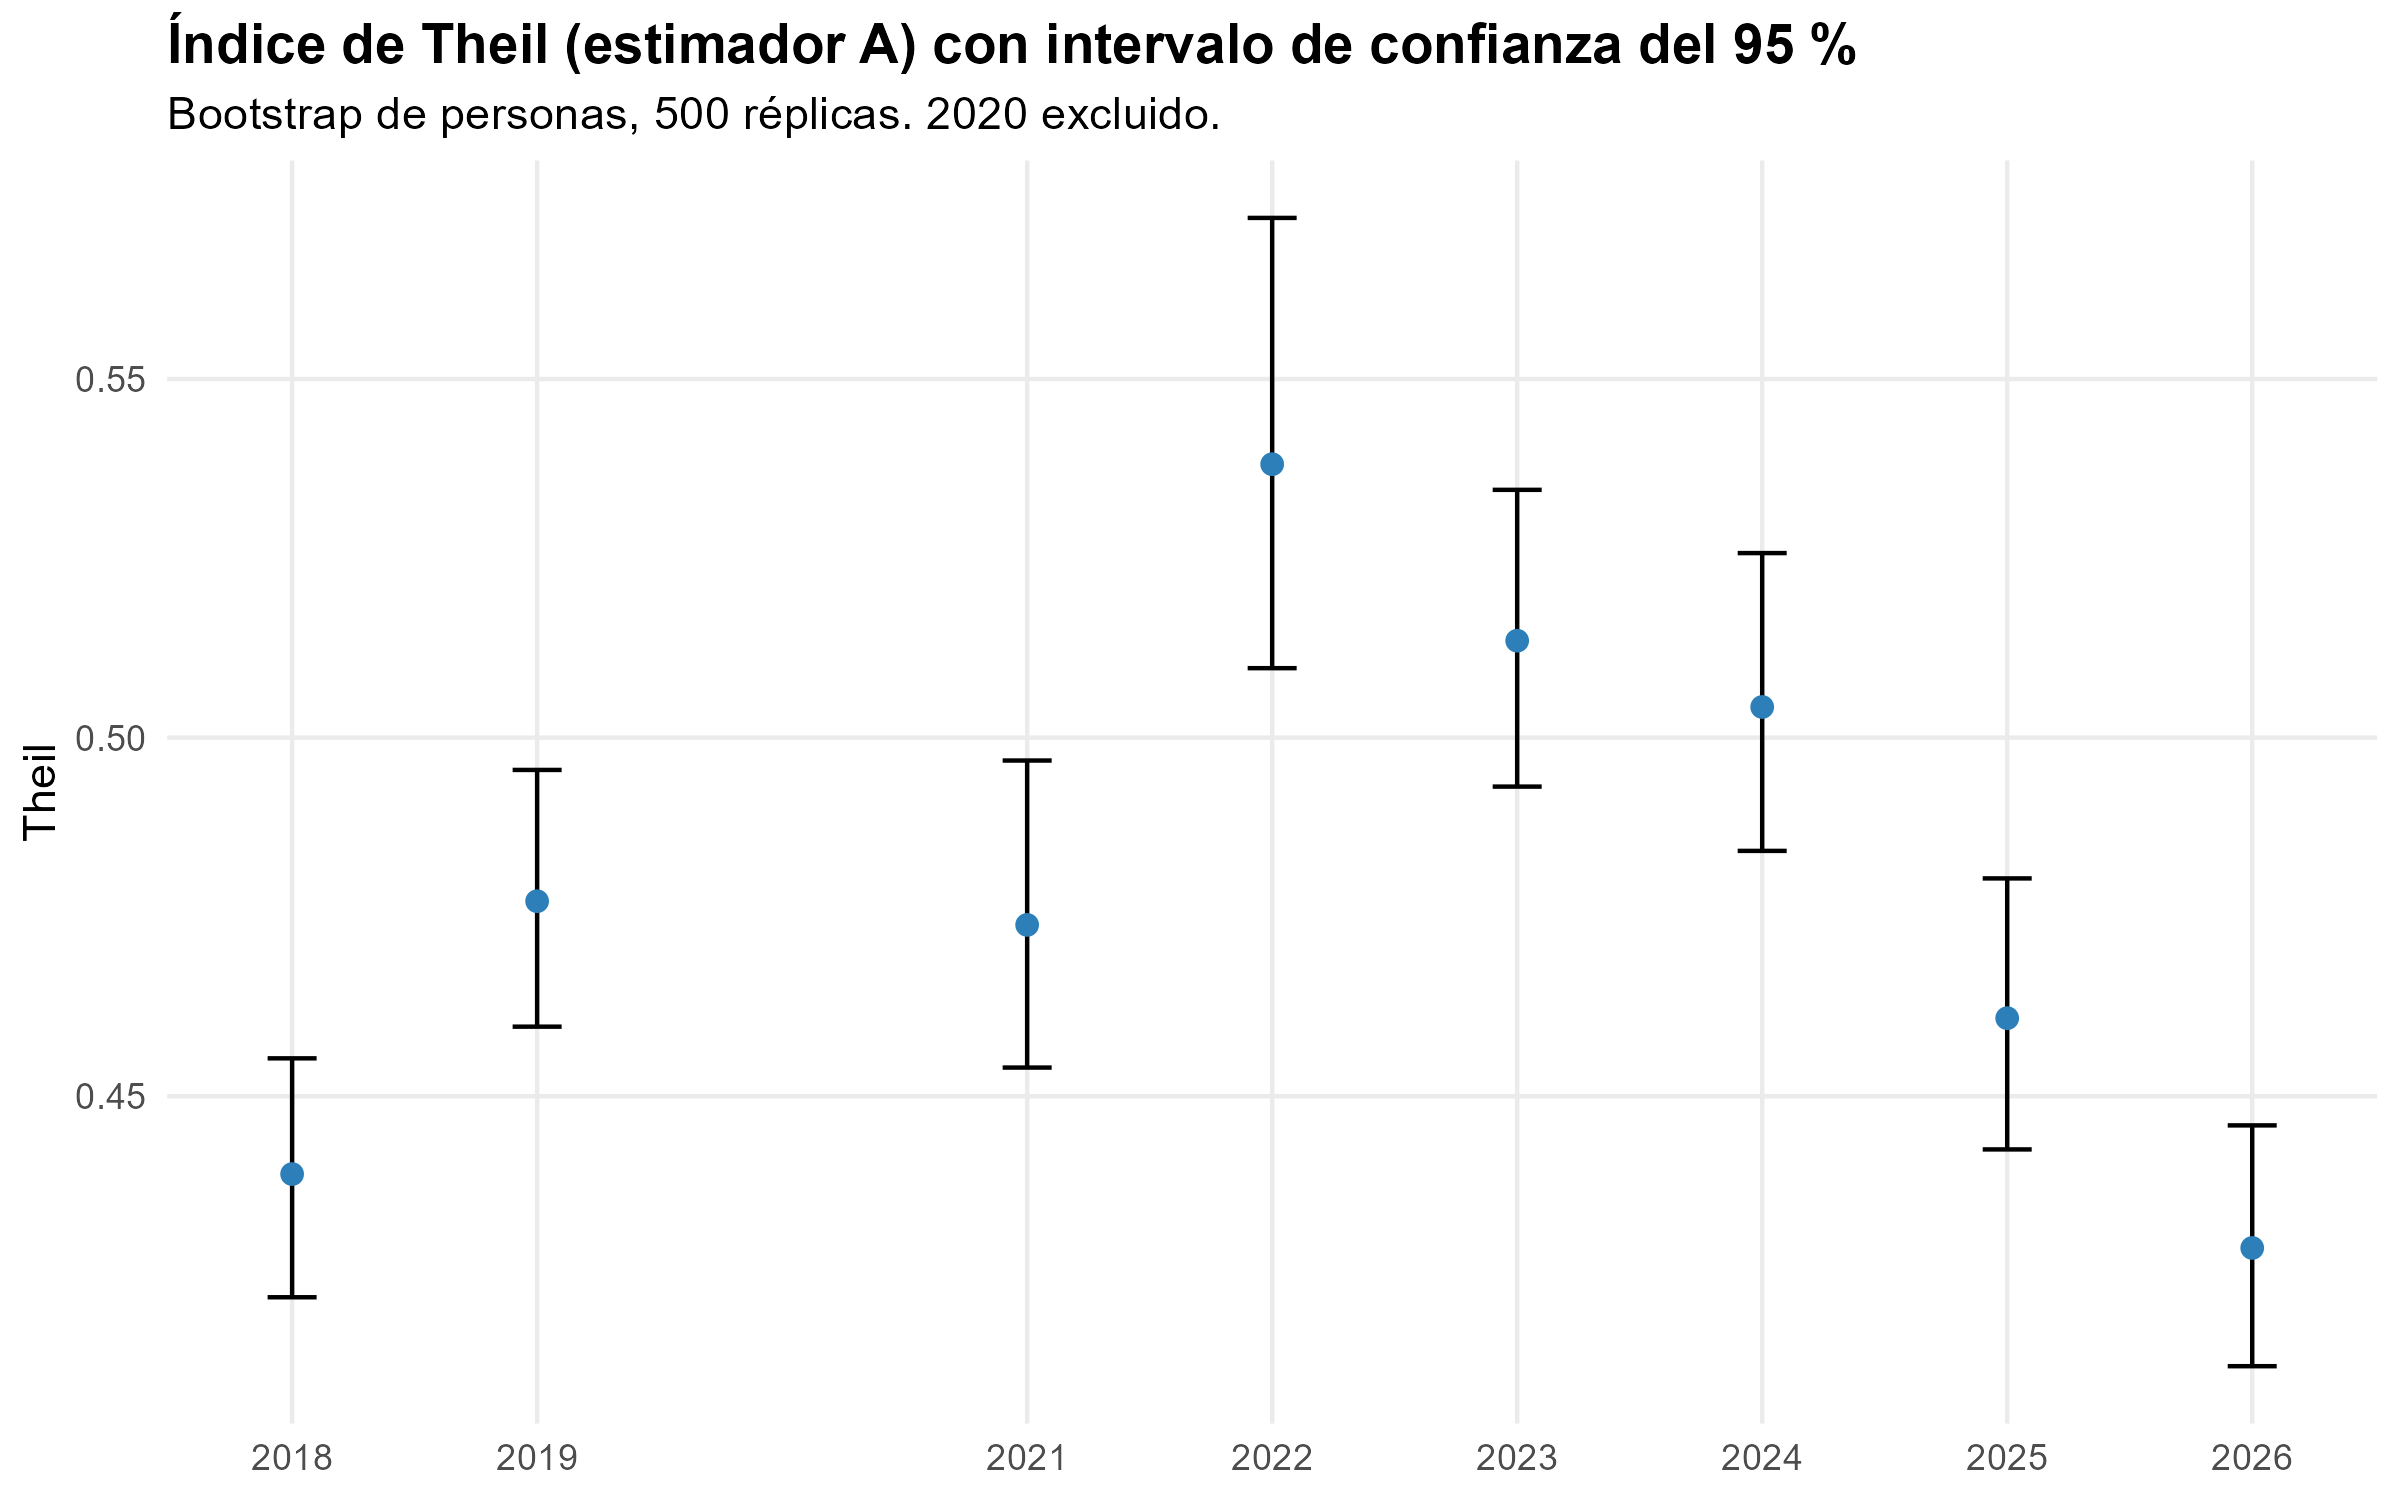
\includegraphics[height=0.8\textheight]{fig_bootstrap_ic.png}
\end{frame}

\begin{frame}{¿Qué explica la desigualdad? (H2)}
  \centering
  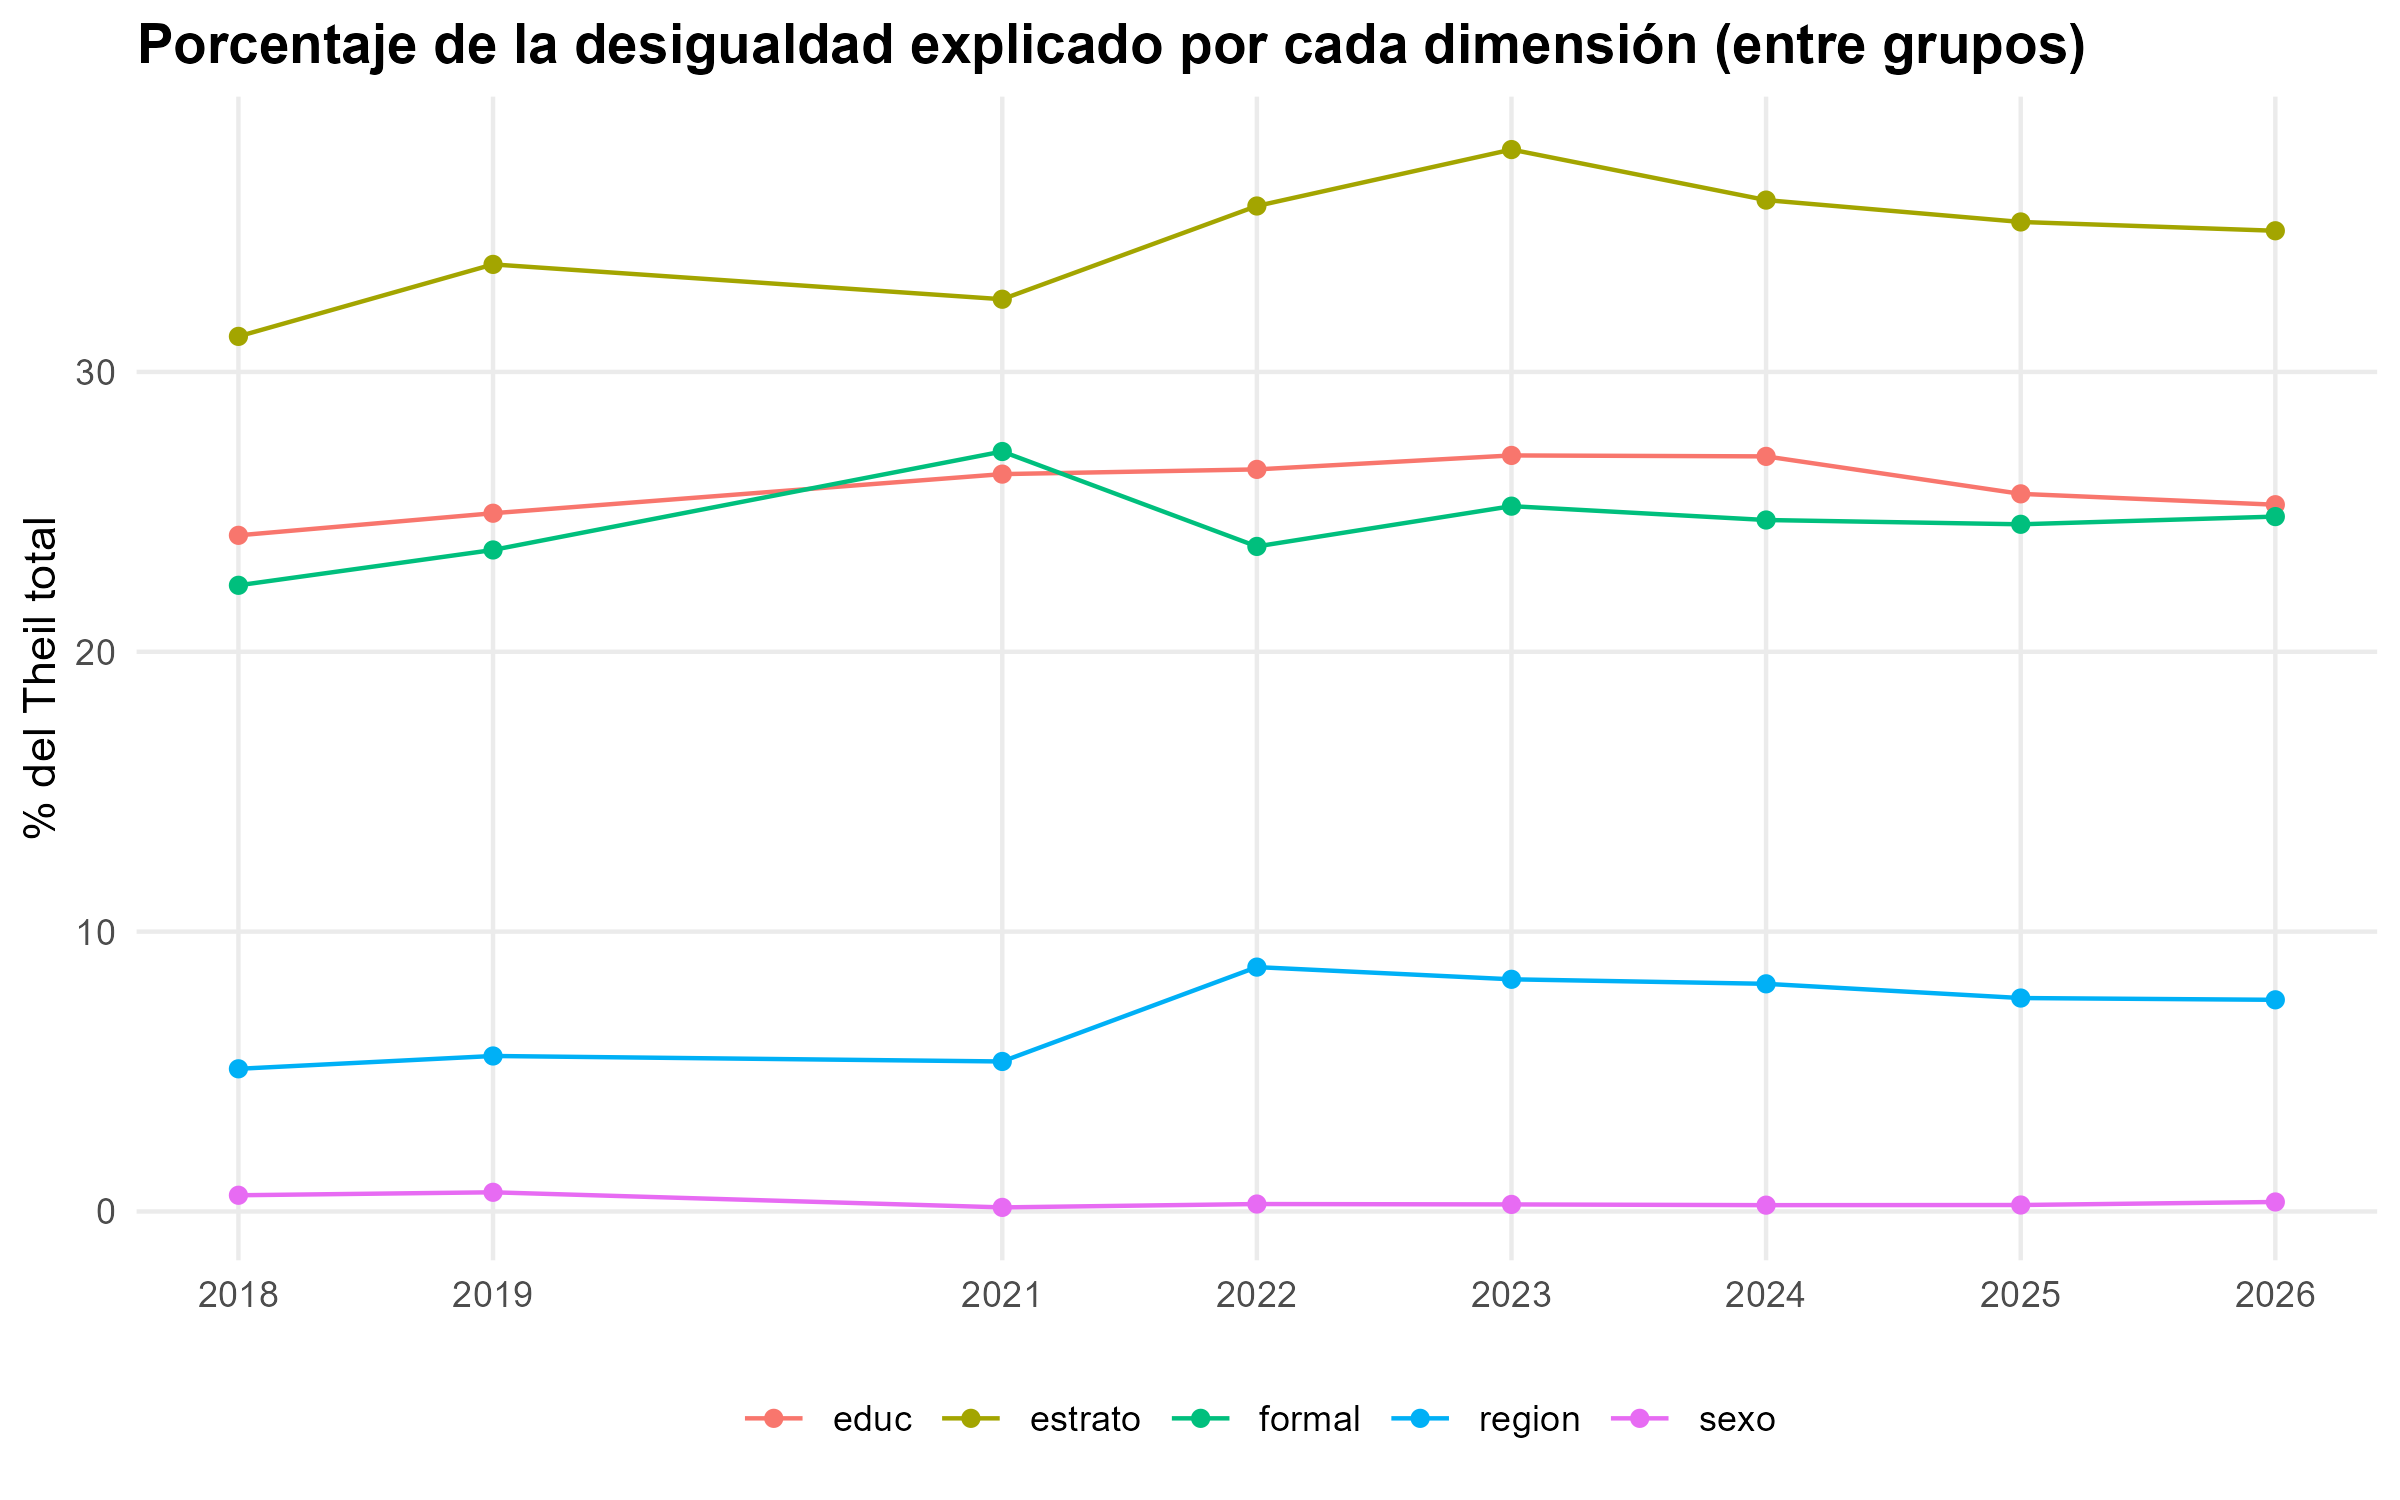
\includegraphics[height=0.8\textheight]{fig_descomposicion.png}
\end{frame}

\begin{frame}{Conclusiones}
  % TODO: tres viñetas
\end{frame}

\begin{frame}[allowframebreaks]{Referencias}
  \nocite{*}
  \printbibliography[heading=none]
\end{frame}

\end{document}
